\section{Übung - JSON}
\label{sec:uebung_10}
Lese die Datei orderdata.sql ein. Diese legt die unten aufgeführte Tabelle weborders an, in der Kundenbestellungen im JSON-Format gespeichert werden.

\begin{figure}[H]
  \centering
  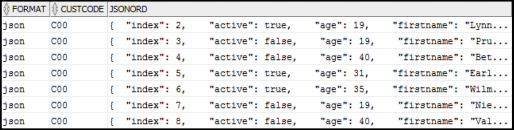
\includegraphics[width=1\textwidth]{img//uebung_10_-_vorbereitung.png}
  \label{img:uebung_10_-_vorbereitung}
\end{figure}

Jedes JSON-Dokument, in der Spalte jsonord, besitzt folgenden Aufbau:
\inputjson{./data/uebung_10_-_vorbereitung.json}

% ##########################################################################
% ############################### Aufgabe 01 ###############################
% ##########################################################################
\label{subsec:uebung_10.aufgabe_01}
\subsection{Aufgabe}
Erzeuge folgende Bestellübersicht, in der nur Bestellungen aus 2014 berücksichtigt werden.

\begin{figure}[H]
  \centering
  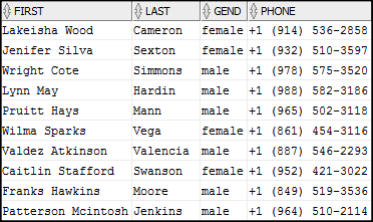
\includegraphics[width=0.75\textwidth]{img//uebung_10_-_aufgabe_01.png}
  \label{img:uebung_10_-_aufgabe_01}
\end{figure}

% ############################### Aufgabe 01A #############################
\label{subsec:uebung_10.aufgabe_01a}
\subsubsection{Aufgabe}
Mithilfe der Funktion json\_value().

\subsubsection*{Lösung}
\label{subsubsec:uebung_10.aufgabe_01a.loesung}
\inputsql{./loesungen/uebung_10/uebung_10_-_aufgabe_01a.sql}


% ############################### Aufgabe 01B #############################
\label{subsec:uebung_10.aufgabe_01b}
\subsubsection{Aufgabe}
Mithilfe der Funktion json\_table().

\subsubsection*{Lösung}
\label{subsubsec:uebung_10.aufgabe_01b.loesung}
\inputsql{./loesungen/uebung_10/uebung_10_-_aufgabe_01b.sql}


% ##########################################################################
% ############################### Aufgabe 02 ###############################
% ##########################################################################
\label{subsec:uebung_10.aufgabe_02}
\subsection{Aufgabe}
Erzeuge folgende Übersicht, die alle Bestellpositionen darstellt.

\begin{figure}[H]
  \centering
  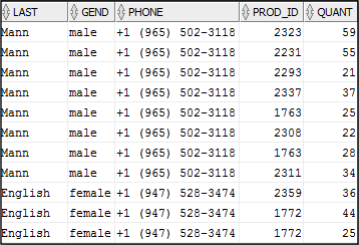
\includegraphics[width=0.6\textwidth]{img//uebung_10_-_aufgabe_02.png}
  \label{img:uebung_10_-_aufgabe_02}
\end{figure}

\subsection*{Lösung}
\label{subsec:uebung_10.aufgabe_02.loesung}
\inputsql{./loesungen/uebung_10/uebung_10_-_aufgabe_02.sql}


% ##########################################################################
% ############################### Aufgabe 03 ###############################
% ##########################################################################
\label{subsec:uebung_10.aufgabe_03}
\subsection{Aufgabe}
Erzeuge eine Übersicht, die für alle Webkunden die abgesetzte Menge je aktivem und nicht aktivem Mitglied sowie die insgesamt abgesetzte Menge zurückgibt.

\begin{figure}[H]
  \centering
  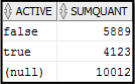
\includegraphics[width=0.25\textwidth]{img//uebung_10_-_aufgabe_03.png}
  \label{img:uebung_10_-_aufgabe_03}
\end{figure}

\subsection*{Lösung}
\label{subsec:uebung_10.aufgabe_03.loesung}
\inputsql{./loesungen/uebung_10/uebung_10_-_aufgabe_03.sql}


% ##########################################################################
% ############################### Aufgabe 04 ###############################
% ##########################################################################
\label{subsec:uebung_10.aufgabe_04}
\subsection{Aufgabe}
Gebe für jeden Monat im Jahr 2015 die Top-2 Webkunden aus, die die meisten Produkte bestellt haben.

\begin{figure}[H]
  \centering
  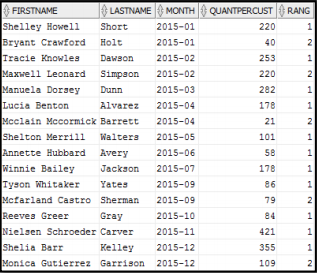
\includegraphics[width=0.6\textwidth]{img//uebung_10_-_aufgabe_04.png}
  \label{img:uebung_10_-_aufgabe_04}
\end{figure}

\subsection*{Lösung}
\label{subsec:uebung_10.aufgabe_04.loesung}
\inputsql{./loesungen/uebung_10/uebung_10_-_aufgabe_04.sql}


% ##########################################################################
% ############################### Aufgabe 05 ###############################
% ##########################################################################
\label{subsec:uebung_10.aufgabe_05}
\subsection{Aufgabe}
Zeige für jeden Webkunden die Anzahl der insgesamt georderten Bestellpositionen.

\subsection*{Lösung}
\label{subsec:uebung_10.aufgabe_05.loesung}
\inputsql{./loesungen/uebung_10/uebung_10_-_aufgabe_05.sql}